% 原书 p.227–p.230（PDF p.235–p.238）
% >>> p235
\section{回到量子上同调（Back to Quantum Cohomology）}

\begin{keytakeaways}
\begin{itemize}
  \item 物理图像：量子上同调环是「带瞬子修正的上同调环」——经典杯积被量子乘积替代，
        后者把所有球面类 $A$ 的三点 Gromov--Witten 不变量作为系数（瞬子数）计入。
  \item 数学工具：小量子乘积（定义 8.7.1）与大量子乘积、Novikov 环中 $T^A$ 的两种约定、
        除子性质与 $\CP^n$ 的显式乘积公式、PSS 映射。
  \item 几何观点：$\Phi_{ijk}=\langle e_i*e_j,e_k\rangle$ 把 §8.6 的势函数的三阶导数与
        量子乘积结构等同起来；PSS 映射 $\Phi_{\mathrm{PSS}}$ 是哈密顿 Floer 同调与量子上
        同调之间的环同构。
  \item 本节结论：$\CP^n$ 中 $c^i*c^j$ 的两分情形公式（$i+j\le n$ 时 $\smile$；否则
        出现 $T^L$ 修正）、$(c)^{*(n+1)}=T^L\cdot1$；辛流形上量子上同调各层信息的
        汇总表（表 8.1）。
\end{itemize}
\end{keytakeaways}

回顾 §8.4 中我们宣布 $\mathrm{QH}^*(M,\omega)$ 带有一个推广了 $H^*(M;\mathbf{k})$ 的
经典杯积的乘积结构 $*$。现在，借助 Gromov--Witten 不变量，我们已准备好给出它的精确定义。

\begin{wdefn}{8.7.1}
给定辛流形 $(M,\omega,J)$ 与 $H^*(M;\Z)$ 的一组基 $\{e_0,\cdots,e_n\}$，在基元素
$e_i,e_j\in\mathrm{QH}^*(M,\omega)$ 上的\textbf{量子乘积}（quantum product）$*$ 定义为
\begin{equation}
  \begin{aligned}
    (e_i*e_j)\big(\operatorname{PD}(e_k)\big)
    &:=\sum_{A\in H_2^S(M)}\mathrm{GW}^M_{A,3}(e_i,e_j,e_k)\,T^A\\
    &=\int_Me_i\cup e_j\cup e_k+(\text{形变部分}),
  \end{aligned}
  \tag{8.52}
\end{equation}
其中第二个等式的第一项来自 $A=0$ 的情形。对一般的输入，乘积由其在基元素上的定义
$\mathbf{k}$-线性地延拓得到。
\end{wdefn}
% [Tutor Note: 重点——(8.52) 第一式与第二式的等价来自例 8.5.4：$A=0$ 的三点 GW 不变量
% 恰是 $\int_Me_i\cup e_j\cup e_k$（经典杯积），其余 $A\ne0$ 的项即「形变部分」。
% 由于 $\operatorname{PD}(e_k)$ 遍历对偶基，(8.52) 唯一确定了 $e_i*e_j$ 这个类。
% 等式 $\Phi_{ijk}=\langle e_i*e_j,e_k\rangle$ 把 §8.6 的势函数三阶导数与量子乘积
% 结构等同起来，因此 WDVV 方程 (8.49) 恰是量子乘积结合律的坐标表述。
% 注意 $T^A$ 的指数是 Novikov 环的元素（也可写成 $T^{\omega(A)}$，见注 8.7.1(i)）。]

\begin{wrem}{8.7.1}
(i) 可以把 (8.52) 中的 $T^A$ 换成 $T^{\omega(A)}$，这取决于我们构造
$\mathrm{QH}^*(M,\omega)$ 时所用的 Novikov 环的约定（见引理 8.1.1 下方的讨论）。

(ii) 定义 8.7.1 只用到 $k=3$ 的 Gromov--Witten 不变量，即三个标记点的约束。当然可以把
类似的表述看作一种乘积结构，但输入为对任意 $k\ge3$ 的 $\mathrm{GW}^M_{A,k}$（见
[223]）。实现这一点有多种方式。例如，固定任意
$\eta\in H^{2m}(M)$（其中 $m\in\N_{\ge1}$），并考虑
\[
  (e_i*_\eta e_j)\big(\operatorname{PD}(e_k)\big)
  :=\sum_{A\in H_2^S(M)}\sum_{l\ge0}\frac{1}{l!}
  \mathrm{GW}^M_{A,l+3}(e_i,e_j,e_k,
  \underbrace{\eta,\cdots,\eta}_{l\text{ 个}})\,T^A .
\]
作为对照，定义 8.7.1 中定义的乘积结构称为\emph{小}量子乘积（small quantum
product），而使用全部 $\mathrm{GW}^M_{A,k}$ 得到的乘积称为\emph{大}量子乘积（big
quantum product）。
\end{wrem}
% [Tutor Note: 小/大量子乘积的区别是本节的易错点：小量子乘积只涉及三点不变量
% $\mathrm{GW}_{A,3}$（即以 $H^*(M)$ 为系数的「经典三点函数」的形变）；大量子乘积则
% 让额外插入 $\eta$（通常是 $H^2$ 类或更一般的高次类）以任意多个进入，等价于把
% 量子乘积写成「以 Novikov 环为系数的形式幂级数运算」。注意注 (ii) 中的 $1/l!$ 与
% (8.47) 中 $\Phi$ 的 $1/k!$ 同源（对称化因子）；$\eta$ 取 $H^{2}$ 类时，
% 由除子性质可进一步简化。]
% >>> p236

\begin{wexam}{8.7.1}
取辛流形 $(M,\omega)=(\CP^n,\omega_{\mathrm{FS}})$、$A=dL$，基为
$H^*(\CP^n;\Z)=\{1,c,c^2,\cdots,c^n\}$。则 $c^i$ 与 $c^j$ 的乘积可写为
\[
  (c^i*c^j)\big(\operatorname{PD}(c^k)\big)
  =\int_{\CP^n}c^i\cup c^j\cup c^k
  +\sum_{d\ge1}\mathrm{GW}^M_{dL,3}(c^i,c^j,c^k)\,T^{dL},
\]
其中次数条件意味着 $2i+2j+2k=2n+2d(n+1)+2\cdot3-6$，即
\[
  i+j+k=n+d(n+1)\quad(\le3n).
\]
这意味着 $d$ 的唯一正取值为 $d=1$，此时 $i+j+k=2n+1$。例如，有
\[
  \mathrm{GW}^M_{L,3}(c^n,c^n,c)=\mathrm{GW}^M_{L,2}(c^n,c^n)=1 .
\]
因此，尽管 $c^n\cup c^n\equiv0$，仍有 $c^n*c^n=c^{n-1}T^L$。为计算更多的量子乘积，
我们需要如下事实。

\begin{wfact}{8.7.1}
（[154] 中的例 11.1.12）可以验证
\[
  \mathrm{GW}^M_{L,3}(c^i,c^j,c^k)=
  \begin{cases}
    1 & \text{若 } i+j+k=2n+1,\\
    0 & \text{其他情形}.
  \end{cases}
\]
\end{wfact}

于是，事实 8.7.1 表明
\[
  c^i*c^j=
  \begin{cases}
    c^{i+j} & \text{若 } i+j\le n,\\
    c^{i+j-n-1}T^L & \text{若 } n+1\le i+j\le2n .
  \end{cases}
\]
特别地，对 $(n+1)$ 个因子施行量子乘积 $*$，得到
$c*c*\cdots*c=c*c^n=T^L=T^L\cdot1$。这恰是例 8.4.1 中的 (8.32)。\hspace*{\fill}$//$
\end{wexam}
% [Tutor Note: 这里 $c^i*c^j$ 的两分情形是 $\CP^n$ 小量子上同调环的经典公式：当
% $i+j\le n$ 时量子修正消失，乘积退化为经典杯积 $c^{i+j}$；当 $i+j\ge n+1$ 时
% 出现一个 $T^L$ 因子并把次数降 $n+1$。由此 $c$ 的 $(n+1)$ 次量子幂等于 $T^L$，
% 这正是 $\mathrm{QH}^*(\CP^n)$ 作为 $\Lambda$-代数由 $c$ 与关系
% $c^{n+1}=T^L$ 生成的原因。核对时请留意 $T^L$ 与 $T^{\omega(L)}$ 的约定
% （$\omega(L)$ 是直线类的辛面积，见注 8.7.1(i)）。]

为结束本节，让我们简要提及量子上同调群 $\mathrm{QH}^*(M,\omega)$ 与定理 5.4.1 所引入的
哈密顿 Floer 同调群 $\mathrm{HF}_*(M,\omega,H,J)$ 之间的关系。回顾第 5 章中，哈密顿
Floer 理论是对辛非球面的辛流形建立的（特别地，(5.17) 中的作用量泛函
$\mathcal{A}_H$ 在可缩环路空间上良定义，即不依赖于边界的圆盘，这与注 5.5.5 中的
$\mu_{\mathrm{CZ}}$ 类似）。

为了把这一构造推广到更一般的辛流形族，必须把来自不同边界圆盘的变化编码进去，这导致与
$\pi_2(M)$ 中球面类相联系的、非平凡的附加量——§8.1 中引入的 Novikov 环
$\Lambda^{\mathbf{k},\Gamma_\omega}$ 提供了打包这类信息的自然候选者。换言之，对一般的
辛流形，哈密顿 Floer 同调应当是一个同调理论，由流 $\{\varphi_H^t\}_{t\in[0,1]}$ 的
（可缩）闭哈密顿轨道生成，系数取自 Novikov 环（域）。

与此同时，作为一个上同调理论，量子上同调
$\mathrm{QH}^*(M,\omega)=H^*(M;\mathbf{k})\otimes\Lambda^{\mathbf{k},\Gamma_\omega}$
自然定义在 Novikov 环 $\Lambda^{\mathbf{k},\Gamma_\omega}$ 上。这里可以把
$H^*(M;\mathbf{k})$ 视为 Morse
% >>> p237
上同调群——应用定理 5.1.2 再加上一个对偶与一个域扩张即可。于是，把哈密顿 Floer 同调群
与 Morse 同调群联系起来便成为一个自然的问题。在链复形的层面上，需要把可缩的闭哈密顿
轨道与 Morse 函数的临界点联系起来。

事实上，这一点已被很好地建立起来，这要归功于 Piunikhin--Salamon--Schwarz 的工作
[176]。即存在一个（$\mathbf{k}$-模的）同构
\begin{equation}
  \Phi_{\mathrm{PSS}}:
  \mathrm{HF}_*(M,\omega,H,J)\cong\mathrm{QH}^*(M,\omega).
  \tag{8.53}
\end{equation}
(8.53) 的左端是一般（比如半正的）辛流形所期望的哈密顿 Floer 同调群。$\Phi_{\mathrm{PSS}}$
的构造（通常称为 \textbf{PSS 映射}）遵循与 (5.23) 中 Floer 边界映射、以及 (7.2) 中
Floer 延拓映射相同的精神。具体地说，它数的是这样的伪全纯柱面：其一端渐近于一条可缩的
闭哈密顿轨道，另一端渐近于 $(M,\omega)$ 上某个 Morse 函数的临界点（示意图形见图 8.5）。

\begin{figure}[htbp]
  \centering
  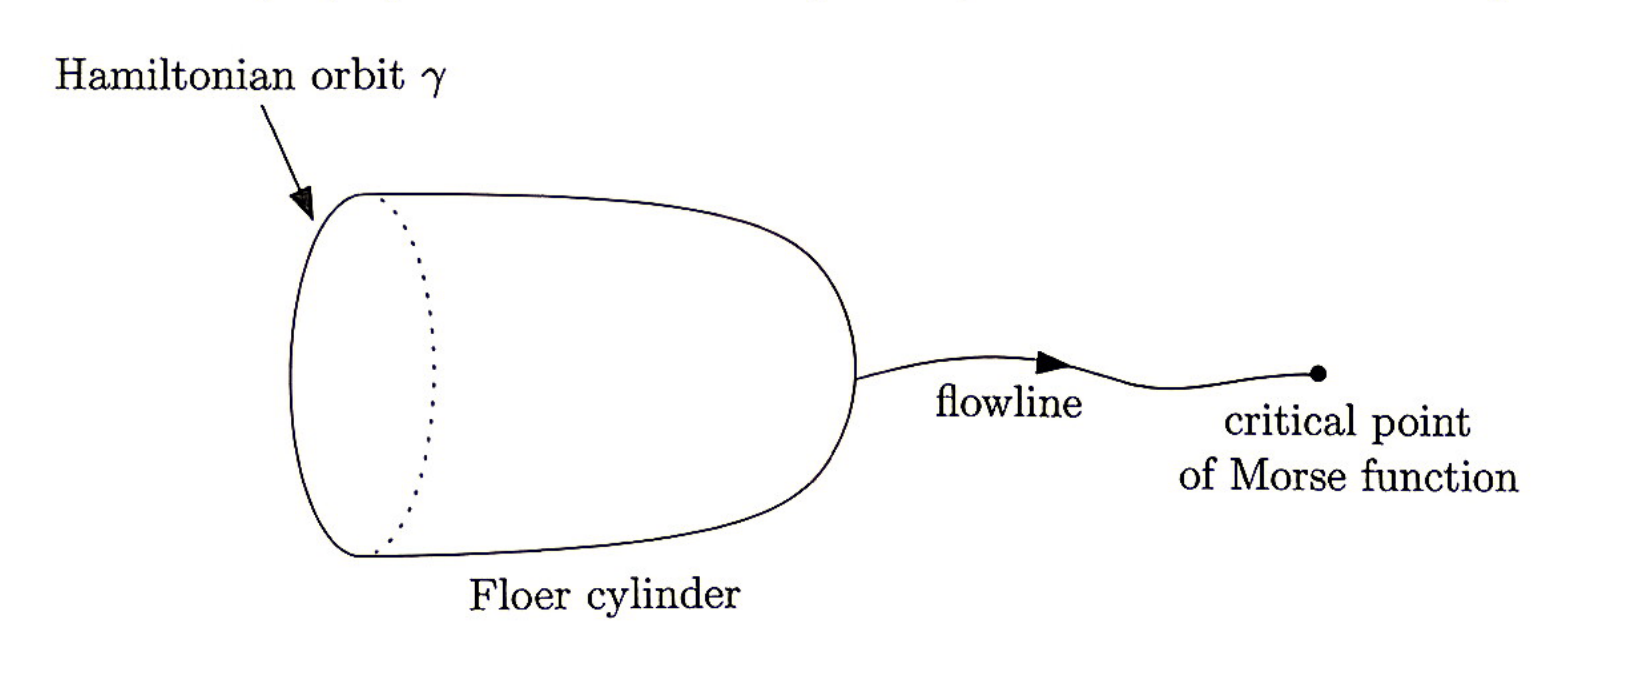
\includegraphics[width=0.82\linewidth]{figures/fig_p237_1.png}
  \caption*{图 8.5\quad 从可缩哈密顿轨道到临界点（原书 p.229, Figure 8.5；PDF p.237）}
\end{figure}

此外，映射 $\Phi_{\mathrm{PSS}}$ 还是一个环同构！这意味着除了定义 8.7.1 中引入的、
位于 (8.53) 右端的量子乘积 $*$ 之外，(8.53) 左端的哈密顿 Floer 同调群上也存在一个
乘积结构，称为\emph{裤子乘积}（pair-of-pants product，示意图形见图 8.6）。关于这一
课题的进一步阅读，见 [154] 第 12.2 节。

还有一点需要强调：若忽略（或回避）作用量泛函 $\mathcal{A}_H$ 在
$\mathrm{HF}_*(M,\omega,H,J)$ 上的良定义性问题，那么哈密顿 Floer 同调的正确的定量视角
是转到 (8.53) 的右端，并使用 §8.2 中 $\mathrm{QH}^*(M,\omega)$ 上的过滤函数 $\ell$
——此时它被视为有限维的 $\Lambda^{\mathbf{k},\Gamma_\omega}$-模。
% [Tutor Note: PSS 映射 $\Phi_{\mathrm{PSS}}$ 是连接「辛拓扑」与「经典拓扑」的桥梁：
% 它把 Floer 同调（由哈密顿轨道生成，依赖 $J$ 与 $H$）与量子上同调（只依赖 $M$ 与
% $\omega$ 的上同调数据）等同起来，且保持环结构（量子乘积 $\leftrightarrow$
% 裤子乘积）。证明的关键是数「一端哈密顿轨道、一端 Morse 临界点」的伪全纯柱面，
% 并对 $J$、$H$、Morse 函数作通有选取以得到横截性。若想核实文献，见
% Piunikhin--Salamon--Schwarz, *Symplectic Floer--Donaldson theory and quantum
% cohomology*, C. R. Acad. Sci. Paris 1996。另注：$\Lambda^{\mathbf{k},\Gamma_\omega}$
% 的 $\Gamma_\omega$ 是 $\omega$ 作用在球面类上取值所生成的群，这是 Novikov 环
% 与辛结构的耦合之处。]

最后，给定辛流形 $(M,\omega)$，让我们总结本章中我们探讨过的关于量子上同调群
$\mathrm{QH}^*(M,\omega)$ 的各种视角，这些视角展示了从它之中提取出的丰富信息。

% >>> p238
\begin{figure}[htbp]
  \centering
  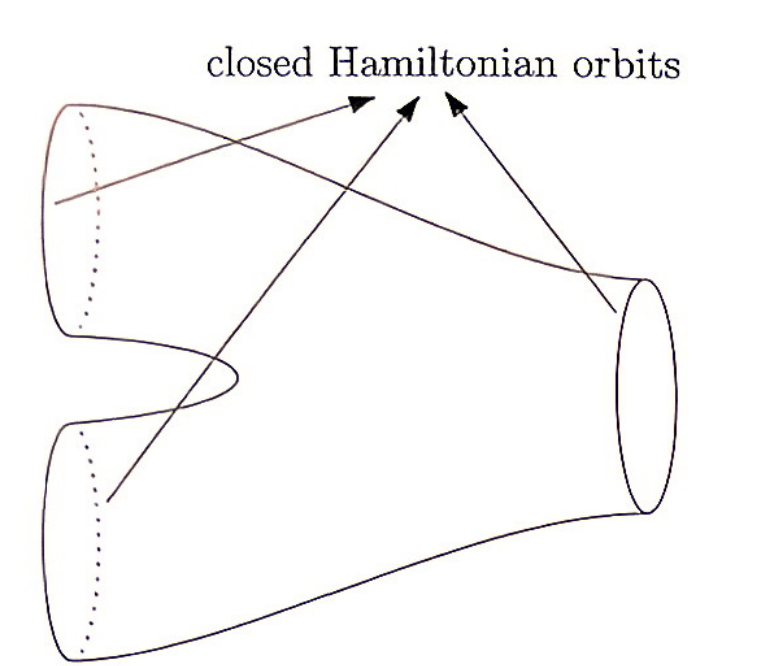
\includegraphics[width=0.42\linewidth]{figures/fig_p238_1.png}
  \caption*{图 8.6\quad 裤子乘积（原书 p.230, Figure 8.6；PDF p.238）}
\end{figure}

\begin{table}[htbp]
  \centering
  \caption*{表 8.1\quad 从 $\mathrm{QH}^*(M,\omega)$ 读出的数据及其应用
  （原书 p.230 无编号表；PDF p.238）}
  \begin{tabular}{@{}p{0.34\linewidth}p{0.56\linewidth}@{}}
    \toprule
    从 $\mathrm{QH}^*(M,\omega)$ 读出的数据 & 在拓扑、几何与动力学中的应用\\
    \midrule
    Novikov 环或 Novikov 域 & 赋值（定义过滤）、非阿基米德线性代数\\
    量子乘积结构 & 定义 Gromov--Witten 不变量（数曲线）\\
    上同调部分的 Morse 解释 & 等同于哈密顿 Floer（上）同调的一个代数\\
    代数结构（域分裂等） & 控制过滤结构与（哈密顿）动力学\\
    \bottomrule
  \end{tabular}
\end{table}
% [Tutor Note: 这张表是本章的总结，也点出了「定量」辛几何的三条主线：Novikov 环的
% 赋值给出过滤（即 §8.2 的 $\ell$，进而给出条形码/持续模）；量子乘积结构对应曲线
% 计数（Gromov--Witten 不变量）；Morse 解释对应 Floer 理论。术语依据：valuation 译
% 「赋值」（非阿基米德意义下），non-Archimedean linear algebra 译「非阿基米德线性
% 代数」；Morse 与 Floer 均按全书统一保留拉丁字母。]
